\documentclass[letterpaper]{article}
\usepackage[submission]{aaai2027}
\usepackage[hyphens]{url}
\usepackage{graphicx}
\urlstyle{rm}
\def\UrlFont{\rm}
\usepackage{natbib}
\usepackage{caption}
\frenchspacing
\usepackage{amsmath,amssymb,amsfonts}
\usepackage{booktabs}
\usepackage{multirow}
\usepackage{array}
\usepackage{tabularx}
\usepackage{colortbl}
\usepackage{xspace}
\usepackage{algorithm}
\usepackage{algorithmic}
\usepackage{float}
\usepackage{placeins}
\pdfinfo{
/TemplateVersion (2027.1)
}

\setcounter{secnumdepth}{2}
\captionsetup{font=small,labelfont=bf,labelsep=colon}
\setlength{\textfloatsep}{8pt plus 2pt minus 2pt}
\setlength{\floatsep}{7pt plus 2pt minus 2pt}
\setlength{\intextsep}{7pt plus 2pt minus 2pt}
\setlength{\abovecaptionskip}{4pt plus 1pt minus 1pt}
\setlength{\belowcaptionskip}{2pt plus 1pt minus 1pt}
\renewcommand{\arraystretch}{1.10}
\definecolor{headerrow}{RGB}{239,243,248}
\definecolor{rghlirow}{RGB}{229,245,237}
\definecolor{controlrow}{RGB}{246,248,251}
\definecolor{cautionrow}{RGB}{255,248,226}
\newcolumntype{Y}{>{\raggedright\arraybackslash}X}
\newcommand{\tblhdr}{\rowcolor{headerrow}}

\newcommand{\method}{\emph{residual-guided hypothesis-language induction}\xspace}
\newcommand{\methodshort}{\textsc{RG-HLI}\xspace}
\newcommand{\uhk}{\textsc{UHK}\xspace}
\newcommand{\mek}{\textsc{MEK}\xspace}
\newcommand{\react}{\textsc{ReAct}\xspace}
\newcommand{\codeact}{CodeAct\xspace}
\newcommand{\gptmini}{GPT-4o-mini\xspace}
\newcommand{\gptfour}{GPT-4o\xspace}
\newcommand{\hms}{\ensuremath{\mathrm{HMS}}\xspace}
\newcommand{\sa}{\ensuremath{\mathrm{SA}}\xspace}
\newcommand{\sr}{\ensuremath{\mathrm{SR}}\xspace}
\newcommand{\ver}{\ensuremath{\mathrm{VER}}\xspace}
\newcommand{\fileid}[1]{\texttt{\small\detokenize{#1}}}
\title{Residual-Guided Hypothesis Language Induction for Scientific Reasoning with Small Language Models}

\author{Anonymous Submission}
\affiliations{}

\begin{document}
\maketitle
\raggedbottom

\begin{abstract}
Scientific reasoning with small language models is limited not only by final
answer verification, but by the earlier problem of constructing the right
hypothesis space before the answer is known. Recent agentic methods improve
long-horizon behavior by adding tool use, reflection, search, and executable
actions. But a structural gap remains: failures are usually stored as text or
trajectory history, so the system does not explicitly change the hypothesis
language used to generate the next scientific artifact. We address this with
two ideas. First, every task is represented through a shared typed hypothesis
state containing answer slots, evidence contracts, executable artifacts,
validators, and residuals. Second, repeated validation failures are converted
into typed residual classes, from which candidate operators are induced and
promoted only when they improve held-out tasks after a complexity penalty. We
implement these ideas as \methodshort, a residual-guided hypothesis-language
induction system around a \gptmini core. The same state, scoring, residual, and
promotion interface is used on DiscoveryBench, NewtonBench, and UltraHorizon.
Complete runs reach 28.09 HMS on DiscoveryBench, 49.7\% audited symbolic
accuracy on NewtonBench, and 75.36 score on UltraHorizon. Controlled ablations
show that typed contracts, answer-slot closure, protocol satisfaction, and
residual-conditioned operator promotion explain distinct parts of the gain.
The results support a narrow mechanism-level claim: small models reason more
effectively when hypothesis construction is externalized as typed, executable,
residual-aware language growth rather than sampled only as free-form prose.
\end{abstract}

\section{Introduction}

Scientific discovery tasks ask an agent to do more than answer a question. The
agent must decide what should be measured, what kind of relation is plausible,
which variables play stable roles, and when a proposed explanation has been
falsified. Recent benchmarks make this distinction explicit. DiscoveryBench
casts data-driven discovery as hypothesis search over real datasets and
metadata \citep{discoverybench}. NewtonBench evaluates interactive scientific
law discovery rather than static curve fitting \citep{newtonbench}.
UltraHorizon stresses long-horizon partially observable exploration
\citep{ultrahorizon}. Across these settings, the bottleneck is often not final
verification but the construction of a useful hypothesis space before the
answer is known.

This bottleneck is especially sharp for small language models. Standard
inference-time scaffolds extend the trajectory: \react interleaves reasoning
and actions \citep{react}, Reflexion and Self-Refine add verbal feedback
\citep{reflexion,selfrefine}, Tree-of-Thoughts and LATS search over reasoning
branches \citep{tot,lats}, and \codeact uses executable code as the action
interface \citep{codeact}. These methods improve many agent tasks, but they
still largely rely on the model to propose the intermediate concepts that make
the search fruitful. If the model never represents the task in the right
coordinates, more attempts can simply explore a larger set of wrong programs.

\methodshort starts from a different premise: hypothesis generation should be treated
as an external, executable induction problem, not as a longer natural-language
trace. A scientific hypothesis is represented as an artifact with typed holes,
evidence contracts, executable measurements, validation tests, and residuals.
The language model proposes local moves, but the environment closes uncertain
parts whenever possible. For example, instead of asking the model to guess a
complete law or discovery statement, the system asks which roles must be filled,
which measurement can identify each role, which residual remains after
execution, and which operator would make that residual simpler on future tasks.

The central object in \methodshort is a shared hypothesis state, \textsc{HypothesisContext}.
It is read and written by heterogeneous components: a universal hypothesis
kernel, evidence-contract compiler, estimand synthesizer, role canonicalizer,
coordinate-probe engine, metamorphic verifier, and residual compiler. This is
not a transcript memory. It is a typed state over hypotheses: what has been
measured, which slots have been closed, which answer forms are admissible,
which residuals recur, and which executable operators compress previous
failures. In this respect \methodshort is closer in spirit to library-learning systems
such as DreamCoder \citep{dreamcoder} than to a pure agent loop, but its learned
unit is not a domain-specific program alone. It is a reusable way of
turning an underspecified scientific task into measurable hypothesis objects.
In ReAct-style agents, a failed tool result remains contextual feedback to the
model; in \methodshort, it is mapped to a typed residual whose type constrains the
next admissible executable operators.

The contribution is threefold. First, we formulate small-model scientific
reasoning as \emph{typed executable hypothesis induction}: a sequence of typed
measurements, validations, and residual-conditioned language edits. Second, we
instantiate this formulation as one shared state, scoring, residual, and
promotion interface that is instantiated with interface-specific executable
operator families for tabular discovery, symbolic law induction, and
long-horizon rule discovery. Third, we report full-run evaluations and
mechanism ablations that separate fixed-language executable search from
residual-conditioned language growth. The empirical results show that
externalizing hypothesis generation makes failures local and diagnosable, while
also revealing a clear remaining bottleneck: small models still need richer
mechanisms for generating useful hypothesis representations when the missing
object cannot be reduced to a measurement.

The paper tests a specific mechanism-level hypothesis: small models fail
scientific reasoning tasks when intermediate hypotheses remain untyped strings,
and they improve when those hypotheses become executable objects with typed
slots, validators, and residuals. This makes the claim narrower than general
``agent improvement'' and broader than a benchmark solver: \methodshort is an
interface for changing the hypothesis language available to the model at
inference time.

\section{Preliminaries}

We write a task instance as
\begin{equation}
  x=(q_x,D_x,\mathcal{T}_x,\mathcal{A}_x,S_x).
\end{equation}
Here $q_x$ is the natural-language instruction, $D_x$ denotes observations such
as tables, metadata, traces, or simulator state, $\mathcal{T}_x$ is an optional
tool or environment interface, $\mathcal{A}_x$ is the admissible answer space,
and $S_x:\mathcal{A}_x\rightarrow\mathbb{R}$ is the benchmark evaluator. The
system observes $q_x,D_x,\mathcal{T}_x$, and the admissible output format, but
does not observe the gold answer before producing its response.

A candidate answer may be a prose hypothesis, a symbolic law, a program, a
transition rule, or a structured report. We use $h\in\mathcal{H}_x$ for such a
scientific artifact and $R_x(h)\in\mathcal{A}_x$ for its rendered benchmark
answer. The distinction is useful because an artifact may contain intermediate
objects--variables, relations, measurements, code, or evidence--that are not
directly shown in the final answer string.

Scientific tasks usually constrain the form of a valid artifact. We denote the
task-level constraints by
\begin{equation}
  C_x=\{s_i=(\tau_i,d_i,\nu_i)\}_{i=1}^{k},
\end{equation}
where $\tau_i$ is a slot type, $d_i$ describes the required evidence or answer
component, and $\nu_i$ is a local validity predicate when one is available.
These constraints describe the task, not any particular solver. They specify
which parts of an artifact must be grounded before the rendered answer can be
considered valid.

Let $E_x(h)$ denote evidence that can be obtained from the observed interface:
statistics computed from a dataset, a fitted symbolic expression, a simulator
trace, a tool result, or a replay check. When an artifact violates a constraint
or fails an available check, we write the discrepancy as a residual
\begin{equation}
  \rho=(\tau_\rho,\ell_\rho,c_\rho,e_\rho,v_\rho),
\end{equation}
where $\tau_\rho$ is the residual type, $\ell_\rho$ is its location in the
artifact or trace, $c_\rho\in C_x$ is the relevant constraint, $e_\rho$ is the
supporting evidence, and $v_\rho$ is the failed check or validator. This
notation only records what failed; later sections describe how residuals are
used by the proposed system.

A hypothesis language is a finite typed language
\begin{equation}
  L=(\mathcal{Y},\mathcal{O}),
\end{equation}
where $\mathcal{Y}$ is a set of artifact and slot types, and $\mathcal{O}$ is a
set of executable typed operators. For a task $x$, the language induces the
search space $\mathcal{H}_x(L)\subseteq\mathcal{H}_x$ of artifacts that can be
constructed and checked using those types and operators.

We use $\mathcal{M}$ for an abstract hypothesis state: a record of the current
contract, candidate artifacts, closed slots, evidence, and residuals. At this
level it is only a notational object. A language operator is any typed
executable transformation of the form
\begin{equation}
  O:\mathcal{M}\times x \rightarrow \mathcal{M}.
\end{equation}
The concrete state representation and operator interface used by \methodshort
are defined in Section~\ref{sec:rghli_method}.

Language induction denotes a sequence of language states
\begin{equation}
  L_0\rightarrow L_1\rightarrow\cdots\rightarrow L_T,
  \qquad
  L_{t+1}=L_t\cup\{o_t^\star\},
\end{equation}
where each added operator expands the set of artifacts that can be constructed
on later tasks. This notation does not specify how $o_t^\star$ is chosen; the
selection mechanism is part of the method.

The objective on each instance is to return $a=R_x(h)$ with high benchmark
score $S_x(a)$. Equivalently, a scientific reasoning system must instantiate
the chain
\begin{equation}
  x \rightarrow C_x \rightarrow h\in\mathcal{H}_x(L)
  \rightarrow R_x(h) \rightarrow S_x(R_x(h)).
\end{equation}
The benchmark evaluator scores only the rendered answer, but the intermediate
objects determine whether a small model can construct a useful answer before
seeing the gold target.

\section{Related Work}

\paragraph{Reasoning-time scaffolds for LLM agents.}
Chain-of-thought prompting showed that exposing intermediate reasoning can
improve large-model problem solving \citep{cot}. Later inference-time methods
make this computation more structured. Self-consistency marginalizes over
sampled reasoning paths \citep{selfconsistency}; least-to-most prompting
decomposes difficult problems into easier subproblems \citep{leasttomost};
\react couples reasoning traces with actions \citep{react}; Reflexion and
Self-Refine use feedback to revise later attempts
\citep{reflexion,selfrefine}; Tree-of-Thoughts and LATS make the search tree
explicit \citep{tot,lats}; STaR turns successful generated rationales into
training data \citep{star}; and \codeact unifies tool use around executable
Python actions \citep{codeact}. These methods are closest to \methodshort at
the level of execution and iterative correction, but they do not by themselves
define what a scientific hypothesis object is. \methodshort uses the same broad
agentic insight--interleave model calls with external computation--but makes
the persistent unit a typed hypothesis state rather than a reasoning
transcript.
This distinction matters when the model's blind spot is representational. If a
model does not propose the right variables, coordinates, answer form, or
transition clauses, additional sampled traces can preserve the same missing
object. \methodshort instead makes the missing object part of the state: a hole or
residual that later operators can target.

\paragraph{Self-optimizing language-model pipelines.}
DSPy treats LM programs as optimizable computational graphs rather than
hand-written prompt strings \citep{dspy}. Self-Discover asks a model to compose
reasoning structures before solving a task \citep{selfdiscover}. Voyager stores
executable skills learned through interaction with Minecraft \citep{voyager}.
PAL and Program-of-Thoughts offload computation to a program runtime once the
model has produced executable intermediate steps \citep{pal,pot}. Toolformer
shows that tool-use decisions themselves can be learned from self-supervised
signals \citep{toolformer}. These systems show that the right unit of
adaptation may be a program, module, executable trace, tool policy, or reusable
skill. \methodshort differs in two ways. First, its stored unit is tied to
scientific evidence: contracts, measurements, residuals, and validators.
Second, promotion is residual-conditioned; an operator is useful only if it
closes typed holes or compresses recurrent failures across tasks.

\paragraph{Program induction and library learning.}
DreamCoder learns a domain language and neural search policy through a
wake-sleep loop over solved and imagined programs \citep{dreamcoder}. Later
library-learning work further explores how abstractions reduce search breadth
and depth, while FunSearch demonstrates that LLM-guided evolutionary program
search can produce new mathematical constructions when candidate programs are
externally evaluated \citep{funsearch}. This line is a major conceptual
ancestor of \methodshort: these systems treat expertise as a changing language
rather than a fixed prompt. The difference is that \methodshort operates in
mixed scientific interfaces where the answer may be prose, a law, or a
transition program, and where holes can often be closed by measurements rather
than by full program synthesis.

\begin{table}[H]
\centering
\caption{Conceptual comparison to DreamCoder-style library learning.}
\label{tab:dreamcoder_compare}
\small
\setlength{\tabcolsep}{4pt}
\begin{tabularx}{\columnwidth}{@{}lYY@{}}
\toprule
\tblhdr
Aspect & DreamCoder-style library learning & \methodshort \\
\midrule
Abstraction source & solved programs & typed validation residuals \\
Learned unit & DSL function / library primitive & operator over hypotheses, evidence, and renderers \\
Promotion signal & compression and synthesis success & held-out gain minus complexity \\
Object of coverage & program behavior & missing roles, contracts, validators, and traces \\
Output type & programs & prose hypotheses, laws, or transition artifacts \\
\bottomrule
\end{tabularx}
\end{table}

\paragraph{Symbolic regression and scientific law discovery.}
Symbolic regression recovers compact formulas from data. AI-Feynman exploits
physics-inspired structure such as symmetry and separability
\citep{aifeynman}; PySR provides a practical evolutionary symbolic-regression
engine for scientific modeling \citep{pysr}. NewtonBench moves beyond static
formula fitting by requiring interactive rediscovery of shifted physical laws
\citep{newtonbench}. \methodshort borrows the insistence on executable hypotheses, but
does not assume that every task reduces to equation recovery. Its coordinate
probes are one operator family inside a broader hypothesis-state kernel.

\paragraph{Causal and experimental-design perspectives.}
Scientific hypotheses are not merely predictors; they make claims about stable
relations under interventions, environments, or perturbations. Structural
causal models formalize this distinction \citep{pearl}, invariant prediction
uses stability across environments to identify causal structure
\citep{invariant}, and Bayesian experimental design studies how to choose
measurements that maximize information \citep{bed}. \methodshort is not a causal
discovery algorithm, but it adopts the same discipline: a hypothesis must state
what evidence would support it, what transformation should preserve it, and
what residual would falsify or refine it.

\paragraph{Automated scientific-discovery agents.}
Recent systems aim to automate larger pieces of the research lifecycle. The AI
Scientist frames end-to-end machine-learning research as an agentic loop over
idea generation, code, experiments, analysis, and writing
\citep{aiscientist,aiscientistnature}. Auto-Bench evaluates scientific
discovery as interactive causal-structure recovery \citep{autobench}, while
AutoDiscovery uses Bayesian surprise to prioritize open-ended data-driven
hypotheses \citep{autodiscovery}. These works motivate the ambition of
autonomous discovery, but they also underline a central risk: if the system's
adaptation is only an outer agent loop, failures remain difficult to localize.
\methodshort addresses a narrower mechanism: the unit that changes over time is
the typed hypothesis language used to generate and validate candidate
scientific artifacts.

\paragraph{Benchmarks for scientific agents.}
DiscoveryBench, NewtonBench, and UltraHorizon expose different faces of the same
problem: the agent must build an internal research object before it can answer.
DiscoveryBench emphasizes data and metadata alignment \citep{discoverybench};
NewtonBench emphasizes interactive law induction and shifted physical laws
\citep{newtonbench}; UltraHorizon emphasizes long-horizon memory, tool use, and
partial observability \citep{ultrahorizon}. We use these benchmarks not as
separate engineering targets but as probes of whether one hypothesis-state
representation can support multiple scientific task interfaces.

\section{\methodshort}
\label{sec:rghli_method}

\subsection{Overview}

\methodshort is a hypothesis-induction kernel around a small language model. The
model is used to propose typed sketches, measurements, and repairs, but the
state of the search is external and executable. The same loop is used for all
benchmarks: compile a contract, generate artifacts, execute measurements,
validate them, store residuals, and occasionally promote a residual pattern into
a new operator. Operators do not pass only text to later calls; they update one
typed context containing contracts, artifacts, evidence, residuals, and
promoted operators.

The design is governed by three invariants. \emph{Typed state}: every useful
intermediate claim must be represented as a slot, artifact, validator, or
residual rather than only as prose. \emph{Executable closure}: whenever a slot
can be identified by a computation or probe, the system closes it by execution
instead of asking the model to guess it again. \emph{Residual discipline}: a
failed hypothesis can expand the operator language only when the residual type
recurs and the proposed operator improves held-out tasks after a complexity
penalty. These invariants are the difference between \methodshort and a longer
self-refinement transcript.

\begin{figure*}[t]
\centering
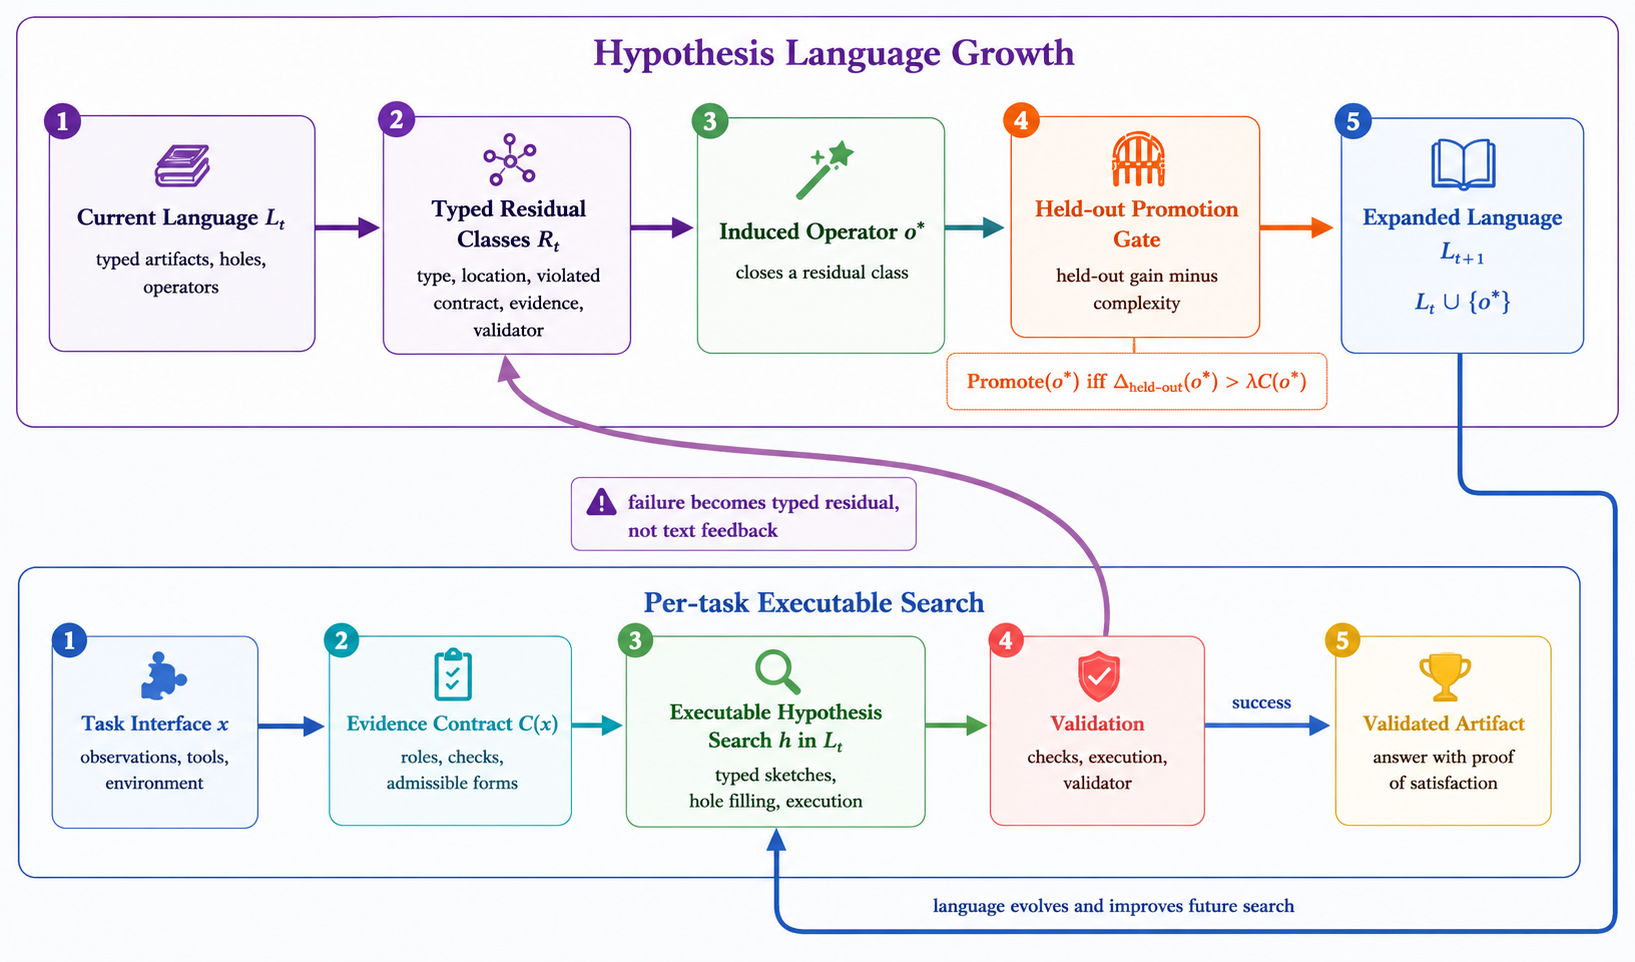
\includegraphics[width=0.98\textwidth]{paper_assets/figures/hypothesis_language_growth_pipeline.png}
\caption{Hypothesis-language growth in \methodshort. The lower loop performs
per-task executable search: a task interface is compiled into evidence
contracts, searched in the current hypothesis language, and validated as an
artifact. Failures are not kept as free-form feedback; they become typed
residual classes. The upper loop turns recurring residual classes into
candidate operators and promotes them only when held-out gain exceeds
complexity, yielding an expanded language for future tasks.}
\label{fig:rghli_architecture}
\end{figure*}

Figure~\ref{fig:language_growth_example} instantiates this mechanism on one
language update: a failed transition artifact becomes a typed residual, several
similar residuals form an ordered-threshold residual class, and the induced
operator expands the next hypothesis language.

\begin{figure*}[t]
\centering
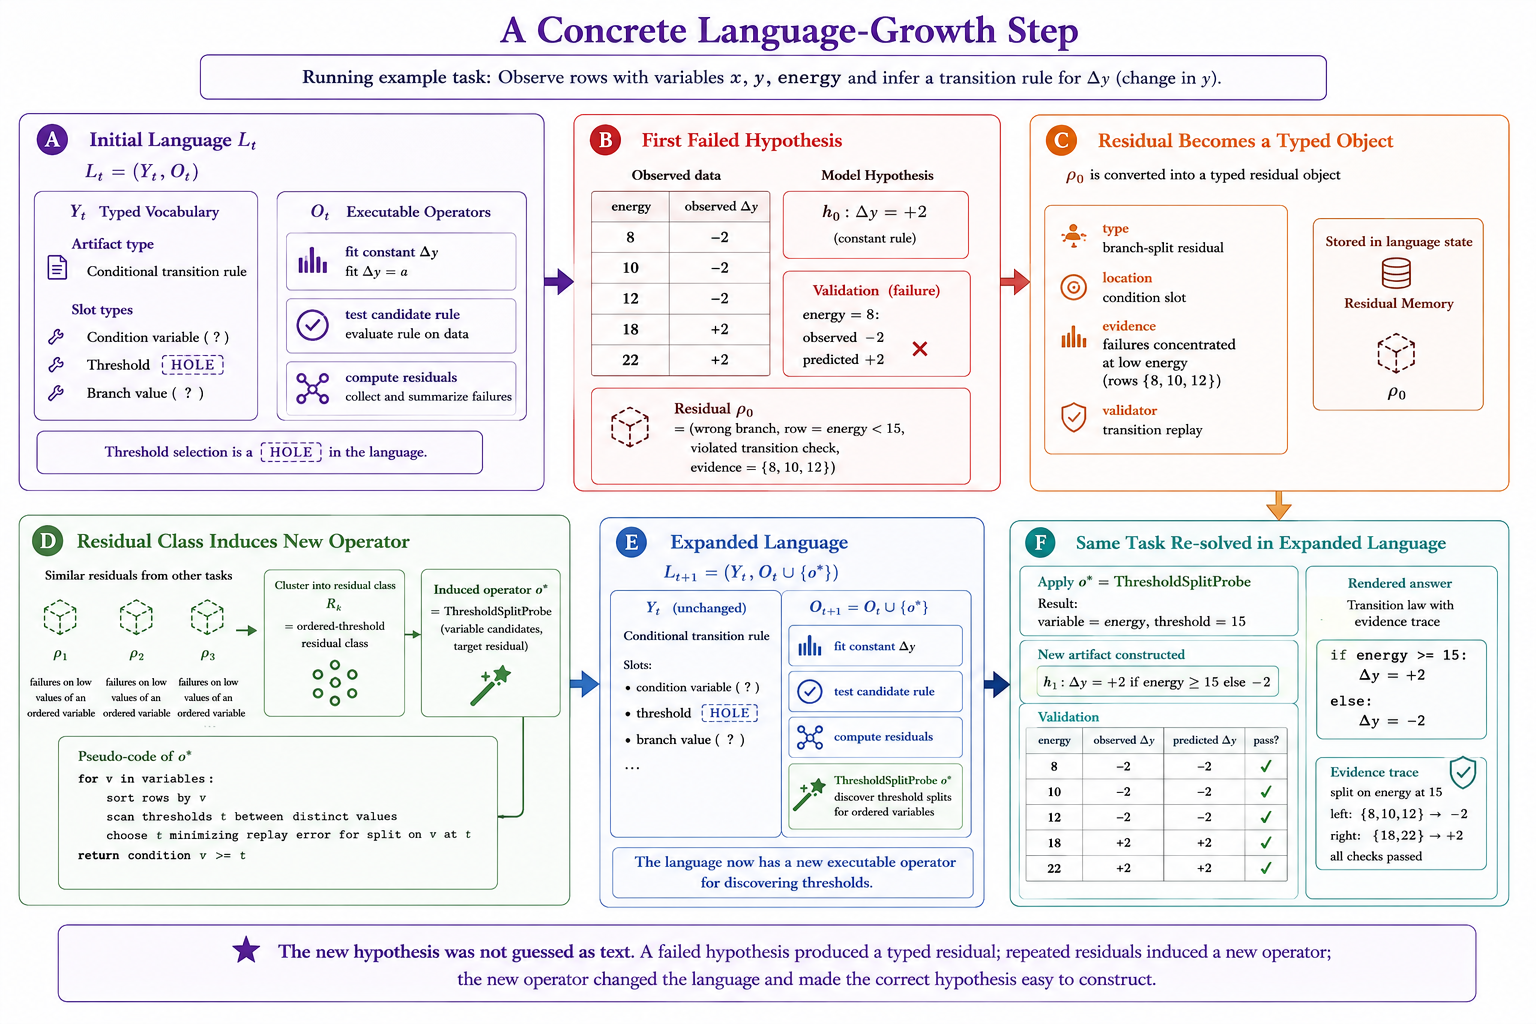
\includegraphics[width=0.98\textwidth]{paper_assets/figures/concrete_language_growth_step.png}
\caption{A concrete hypothesis-language growth step. Starting from a language
that can test transition rules but lacks an operator for discovering ordered
thresholds, a failed artifact produces a typed residual concentrated on
low-energy rows. Similar residuals induce a \textsc{ThresholdSplitProbe}
operator, yielding an expanded language that constructs the correct conditional
transition rule by execution rather than by one-shot textual guessing.}
\label{fig:language_growth_example}
\end{figure*}

\subsection{The \textsc{HypothesisContext}}

For a task $x$, the context is
\begin{equation}
  \mathcal{M}_x=(C,\mathcal{H},\Theta,\mathcal{E},
  \mathcal{R},\mathcal{O},h^\star),
\end{equation}
where $C$ is the evidence contract, $\mathcal{H}$ is the pool of candidate
artifacts, $\Theta$ stores closed typed holes, $\mathcal{E}$ stores executable
evidence, $\mathcal{R}$ stores typed residuals, $\mathcal{O}$ is the active
operator set, and $h^\star$ is the current best answer artifact. All operators
read and write this object. This is the main architectural constraint: every
stage must return a state update, not a private chain of thought.

Each operator $O_j\in\mathcal{O}$ has the same interface,
\begin{equation}
  O_j(\mathcal{M}_x,x) \rightarrow
  \{(h,e,\rho,\Delta\mathcal{M})\},
\end{equation}
where $h$ is a proposed artifact, $e$ is executed evidence, $\rho$ is the typed
residual, and $\Delta\mathcal{M}$ is the state update. This interface is what
makes the system benchmark-independent. A tabular estimand, a symbolic
coordinate probe, and a transition-rule inducer differ internally, but the
kernel only sees artifact, evidence, residual, and update.

\paragraph{Candidate scoring and typed residuals.}
The kernel ranks candidates by a shared energy score:
\begin{equation}
\begin{aligned}
  \operatorname{score}(h)
  ={}& \lambda_E E(h,x)
  + \lambda_C \operatorname{cover}(h,C) \\
  &- \lambda_V V(h,C)
  - \lambda_K K(h).
\end{aligned}
\end{equation}
This objective is Bayesian in motivation--evidence should increase confidence,
while instability and complexity should decrease it--but we do not require a
calibrated likelihood or learned prior. The operational object is the
benchmark-independent energy decomposition and the typed residual emitted when
that score fails. Table~\ref{tab:score_terms} makes the scoring
parameterization explicit. The same decomposition is used across interfaces,
while each operator normalizes its executable evidence to a comparable range
before entering the shared ranking function. The weights were fixed for the
reported runs; sensitivity to these constants remains a target for a larger
calibration study.

\begin{table}[H]
\centering
\caption{Energy terms used by the shared hypothesis kernel.}
\label{tab:score_terms}
\small
\setlength{\tabcolsep}{4pt}
\begin{tabularx}{\columnwidth}{@{}lYcc@{}}
\toprule
\tblhdr
Term & Definition & Range & Weight \\
\midrule
$E$ & executable fit or local score & $[0,1]$ & 24 \\
Cover & contract slots covered & $[0,1]$ & 34 \\
$V$ & metamorphic validation loss & $[0,1]$ & 32 \\
$K$ & operator complexity & $\geq0$ & 2 \\
\bottomrule
\end{tabularx}
\end{table}

\paragraph{End-to-end trace.}
In a NewtonBench-style trajectory, the model does not guess the law directly:
the contract asks for coordinate, exponent, constant, and residual slots; a
sketch $y=c\phi(x)^p$ is executed; residual curvature activates a coordinate
probe; the probe closes the coordinate, exponent, and constant slots; and the
held-out validator accepts the artifact. The
failed first probe changes typed state rather than merely changing the next
prompt.

\subsection{Operators}

\paragraph{Contract compiler.}
The contract compiler maps the input interface to required slots and local
validators. It does not predict the gold answer. It predicts what any valid
answer must make observable: answer type, scope, variables, measurement target,
relation form, and rendering constraints.

\paragraph{Typed-hole closure.}
Instead of asking the model for a complete hypothesis, \methodshort asks for sketches
with typed holes and then closes the holes by small executable probes whenever
possible. For a tabular question, a hole may be an outcome role or a window
operator. For a law-discovery task, it may be a coordinate chart or exponent.
For a sequence task, it may be a state variable or transition clause. Closing a
hole adds an assignment to $\Theta$ and reduces the search space for later
holes.

\paragraph{Executable estimands and coordinate probes.}
The estimand operator creates statistical objects for tabular discovery:
group contrasts, interaction effects, coefficient shifts, multi-item
proportions, and time-window measurements. The coordinate-probe operator
creates compact transformations for laws and rules: log-log fits, affine and
polynomial lifts, ratios, finite differences, thresholds, and simple
state-transition clauses. Both operators produce evidence objects rather than
only prose rationales.

\paragraph{Metamorphic verifier.}
The verifier checks whether the artifact answers the requested question under
transformations that should preserve the object: renaming irrelevant columns,
holding answer form fixed, changing display order, perturbing nuisance values,
or replaying held-out traces. These checks are label-free and therefore
available before benchmark evaluation.

\subsection{Induction Algorithms}

\begin{algorithm}[t]
\caption{Per-task executable search in a frozen hypothesis language}
\label{alg:per_task_search}
\begin{algorithmic}[1]
\REQUIRE task interface $x$, frozen language $L^\star$, budget $B$
\STATE $C \leftarrow \textsc{CompileContract}(x)$
\STATE $\mathcal{M}\leftarrow(C,\emptyset,\emptyset,\emptyset,\emptyset,L^\star,\emptyset)$
\FOR{$t=1$ to $B$}
  \STATE $\mathcal{P}\leftarrow\emptyset$
  \STATE $\mathcal{Q}\leftarrow\textsc{SelectOperators}(\mathcal{M},x,B-t)$
  \FORALL{$O_j\in\mathcal{Q}$}
    \STATE $\mathcal{P}\leftarrow\mathcal{P}\cup O_j(\mathcal{M},x)$
  \ENDFOR
  \FORALL{$(h,e,\rho,\Delta\mathcal{M})\in\mathcal{P}$}
    \STATE update $\mathcal{M}$ with $h,e,\rho,\Delta\mathcal{M}$
    \STATE score $h$ by evidence, coverage, validation, and complexity
    \IF{$h$ improves $h^\star$}
       \STATE $h^\star \leftarrow h$
    \ENDIF
  \ENDFOR
  \IF{$h^\star$ satisfies $C$ and validation checks}
     \RETURN $\textsc{Render}(h^\star,C)$
  \ENDIF
\ENDFOR
\RETURN $\textsc{Render}(h^\star,C)$
\end{algorithmic}
\end{algorithm}

\begin{algorithm}[t]
\caption{Development-time residual-conditioned language induction}
\label{alg:language_induction}
\begin{algorithmic}[1]
\REQUIRE development tasks $\mathcal{D}$, initial language $L_0$, held-out split $\mathcal{D}_{held}$
\STATE $L\leftarrow L_0$, residual buffer $\mathcal{B}\leftarrow\emptyset$
\FORALL{$x\in\mathcal{D}$}
  \STATE run Algorithm~\ref{alg:per_task_search} with language $L$
  \STATE append emitted typed residuals to $\mathcal{B}$
\ENDFOR
\STATE $\mathcal{R}_1,\ldots,\mathcal{R}_k\leftarrow\textsc{ClusterResiduals}(\mathcal{B})$
\FORALL{residual class $\mathcal{R}_i$}
  \STATE $o_i\leftarrow\textsc{SynthesizeOperator}(\mathcal{R}_i)$
  \IF{$o_i$ passes static checks, sandbox execution, and validators}
    \STATE $\Delta_i\leftarrow S_{\mathcal{D}_{held}}(L\cup\{o_i\})-S_{\mathcal{D}_{held}}(L)$
    \IF{$\Delta_i>\lambda K(o_i)$}
      \STATE $L\leftarrow L\cup\{o_i\}$
    \ENDIF
  \ENDIF
\ENDFOR
\RETURN frozen language $L^\star=L$
\end{algorithmic}
\end{algorithm}

The two algorithms run at different time scales. Algorithm~\ref{alg:per_task_search}
is the reported benchmark-time procedure: it searches within a frozen language
$L^\star$ and may store residuals for analysis, but it does not change
$L^\star$ using later test examples. Algorithm~\ref{alg:language_induction}
is the development-time mechanism that turns recurring residual classes into
candidate operators. Candidate operators are generated by the same small-model
code-and-sketch interface used elsewhere in the system, then filtered by static
checks, sandbox execution, validators, and held-out promotion. Human input is
limited to the initial typed operator schema and benchmark interface adapter;
the promoted operator must be selected by the residual-to-operator pipeline and
pass the held-out gate.

\paragraph{Language-growth protocol.}
The promotion step has two modes. During development, residuals may induce
candidate operators, which are promoted only if they improve a held-out
development set after the complexity penalty in Eq.~\eqref{eq:promotion}. For the headline
benchmark runs, the resulting operator language $L^\star$ is frozen before the
reported evaluation. The benchmark score is never used as the promotion signal
for examples later reported as test results. Online adaptation is therefore
limited to per-task hypothesis search in the frozen language, not to changing
the language using future test labels.

\subsection{Residual-Conditioned Operator Promotion}

The residual-extension step is not arbitrary code growth. A residual cluster
$R=\{\rho_1,\ldots,\rho_m\}$ can propose an operator only if it identifies a
repeatable missing transformation. Formally, a candidate operator $O'$ is
promoted when
\begin{equation}
  \Delta(O') =
  \mathbb{E}_{x\sim\mathcal{D}_{held}}
  [S(h^\star_{O'}(x))-S(h^\star(x))]
  -\beta K(O') > 0,
\label{eq:promotion}
\end{equation}
and the improvement is not confined to the task that produced the residual.
This rule is meant to prevent an ever-growing bag of benchmark-specific tricks:
an operator must improve held-out tasks under the same contract and scoring
interface while paying a complexity penalty.

\subsection{Why This Helps Small Models}

\methodshort changes the role of the language model. The model does not need to hold
the entire long-horizon proof in context or invent the final hypothesis in one
sample. It repeatedly proposes local typed objects whose consequences can be
executed. Each closed hole constrains later holes, each verifier rejects an
invalid answer form before final scoring, and each residual becomes a structured
training signal for the outer loop. The intended gain is therefore not more
 verbal reasoning, but a better external search geometry for capacity-limited models.

\section{Experimental Evaluation}

\subsection{Benchmarks and protocol}

We evaluate on three benchmark families that stress different scientific
interfaces while sharing the same central difficulty: the agent must construct
a hypothesis object before it can answer. DiscoveryBench provides real
datasets, metadata, and natural-language discovery goals; the final answer is
scored by Hypothesis Matching Score (HMS) and a consistency-HMS variant.
NewtonBench provides interactive scientific-law discovery tasks in shifted
physical worlds; we report symbolic accuracy over all tasks (SA-all) and over
non-abstained answers (SA-answered). UltraHorizon provides long-horizon
partially observable rule-induction environments; we report the reproduced
paper-style environment score.

The reported system uses a \gptmini core throughout. We use one shared
hypothesis-induction stack: contract compilation, typed-hole closure,
estimand synthesis, coordinate probing, metamorphic validation, and
residual-conditioned promotion. Benchmark adapters expose observations and
accept final artifacts; interface-specific operator families expose measurable
objects appropriate to each environment, but they all write the same
\textsc{HypothesisContext} and are scored by the same evidence, validation,
residual, and complexity rules. We exclude diagnostic ceiling runs that used
task-family measurement bootstraps or hand-engineered rendering fixes.

\paragraph{Reproducibility audit.}
For DiscoveryBench we evaluate the repository real-test task rows using the
benchmark evaluator, producing 239 predictions and 239 scored rows. For
NewtonBench we evaluate the full cross-product of 12 physics domains, three
difficulty levels, three law versions, and three system variants, for 324
symbolic-law tasks. For UltraHorizon we evaluate 32 seeds for each of the
three official environments, for 96 total runs, using the paper-style judge,
hard difficulty, 50-step episodes, and no environment hints or measurement
bootstraps. The row-level outputs are retained for each benchmark, and the main
table is generated only from complete runs with the expected row counts. The
language used in these evaluations is frozen before scoring; residuals from
reported test rows are analyzed after the run and are not used to promote new
operators for later rows in the same headline evaluation.
For UltraHorizon we report both a strict agent-only ablation and the full
\methodshort system. The strict run disables fallback commits, environment
hints, and measurement bootstraps. The full run adds a terminal protocol
controller: it uses only public environment actions to satisfy explicit
terminal preconditions, such as the Bio environment's 50-successful-cross
requirement, before compiling the final artifact from the observed trace. It
does not inspect hidden rules, gold labels, or judge feedback.

\begin{table}[!htbp]
\centering
\caption{Benchmark interfaces and metrics.}
\label{tab:benchmarks}
\small
\setlength{\tabcolsep}{4pt}
\begin{tabularx}{\columnwidth}{@{}lYYY@{}}
\toprule
\tblhdr
Benchmark & Interface & Artifact & Metric \\
\midrule
DiscoveryBench & tables, metadata, goal & hypothesis & HMS / Cons-HMS \\
NewtonBench & simulator, observations & symbolic law & SA-all / SA-answered \\
UltraHorizon & POMDP-style env. & transition rule & score \\
\bottomrule
\end{tabularx}
\end{table}

\subsection{Main full-run results}

Table~\ref{tab:main_results} gives the current full-run results. Each row is a
complete benchmark run under the corresponding native metric. The pattern is
informative rather than uniformly dominant. On DiscoveryBench, \methodshort
improves over the published prompt-level references listed in
Table~\ref{tab:published_refs} under the same HMS scale, while remaining
sensitive to answer rendering and multi-file assembly. On NewtonBench,
\methodshort reaches 49.7\% audited SA-all, 1.9 points above the published
o4-mini reference and below stronger frontier-model agents. On UltraHorizon,
the strict agent-only ablation scores 51.04 without hints, bootstraps, or
fallback commits; the full system scores 75.36 once the terminal protocol
controller is enabled. The split is essential: it shows that model failure under
limited capacity can be procedural rather than conceptual, especially in the Bio
environment.

We therefore make two claims from the table. The first is empirical: the same
\gptmini-core hypothesis kernel produces nontrivial full-run results across
three different scientific interfaces. The second is diagnostic: the failures
concentrate in different residual types across benchmarks, which supports the
use of a shared typed state rather than benchmark-specific prompt repair. We do
not claim that the current operator set dominates all larger-model systems.
Generic direct and \react-style prompting test a different question from
Table~\ref{tab:main_results}: whether longer verbal reasoning alone can explain
the improvement. These baselines do not use \methodshort state or
residual-conditioned operators, so they are treated as separate controls rather
than as variants of the proposed method.

\begin{figure}[t]
\centering
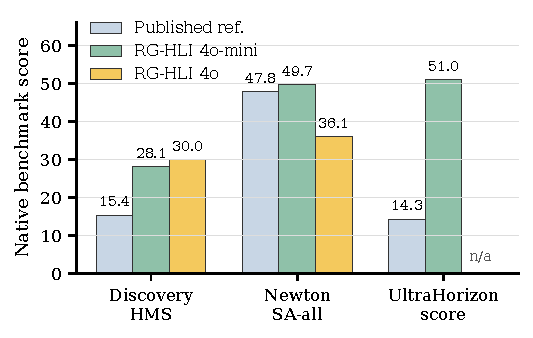
\includegraphics[width=\columnwidth]{paper_assets/figures/main_results_chart.pdf}
\caption{Headline comparison under each benchmark's native metric. Reference
rows are contextual rather than controlled ablations because the published
systems use different models, budgets, and interfaces. The plotted
UltraHorizon \methodshort row is the strict agent-only score; the full
terminal-protocol score is reported separately in
Tables~\ref{tab:main_results} and~\ref{tab:uh_protocol}.}
\label{fig:main_results_chart}
\end{figure}

\begin{table}[t]
\centering
\caption{Full-run \gptmini-core \methodshort results under each benchmark's
native evaluator.}
\label{tab:main_results}
\footnotesize
\setlength{\tabcolsep}{3pt}
\begin{tabularx}{\columnwidth}{@{}lccY@{}}
\toprule
\tblhdr
Benchmark & Tasks & Result & Secondary detail \\
\midrule
DiscoveryBench & 239 & 28.09 HMS & 36.04 consistency-HMS \\
NewtonBench & 324 & 49.7\% SA & 67.1\% SA-answered \\
UltraHorizon & 96 & 75.36 & full: Grid 54.38; Seq 81.25; Bio 90.47 \\
\rowcolor{controlrow}
UltraHorizon & 96 & 51.04 & strict: Grid 59.38; Seq 93.75; Bio 0.00 \\
\bottomrule
\end{tabularx}
\end{table}

\begin{table}[t]
\centering
\caption{Published references under each benchmark's native metric. Reference
systems are not all matched by model, budget, or protocol, so they provide
context rather than controlled ablations. Shaded rows mark the
\methodshort configuration evaluated here.}
\label{tab:published_refs}
\footnotesize
\setlength{\tabcolsep}{3pt}
\begin{tabularx}{\columnwidth}{@{}lYc@{}}
\toprule
\tblhdr
Benchmark & System / core model & Score \\
\midrule
DiscoveryBench & GPT-4o ReAct / GPT-4o & 15.4 HMS \\
DiscoveryBench & CodeGen / GPT-4-preview & 16.3 HMS \\
DiscoveryBench & Reflexion / GPT-4 family & 24.5 HMS \\
\rowcolor{rghlirow}
DiscoveryBench & \methodshort / \gptmini & 28.09 HMS \\
\addlinespace[2pt]\midrule
NewtonBench & Vanilla agent / GPT-5 & 75.9\% SA \\
NewtonBench & Vanilla agent / Gemini-2.5-Pro & 65.4\% SA \\
NewtonBench & Vanilla agent / o4-mini & 47.8\% SA \\
\rowcolor{rghlirow}
NewtonBench & \methodshort / \gptmini & 49.7\% SA \\
\addlinespace[2pt]\midrule
UltraHorizon & Best free-step LLM / reported best & 14.33 \\
UltraHorizon & Human / human & 26.52 \\
\rowcolor{rghlirow}
UltraHorizon & \methodshort strict agent-only / \gptmini & 51.04 \\
\bottomrule
\end{tabularx}
\end{table}

\subsection{Full-run mechanism evidence}

The headline table alone would under-specify the central novelty: typed
contracts and executable probes could improve a fixed hypothesis language
without demonstrating induction of a better language. We therefore separate
mechanism controls from the leaderboard. Table~\ref{tab:language_growth}
uses only complete benchmark runs or complete official grids. Each control
removes a language-growth or residual-handling mechanism while preserving the
same benchmark interface and native evaluator.

\begin{table}[t]
\centering
\caption{Full-run mechanism controls. Rows are complete runs under the native
benchmark metric.}
\label{tab:language_growth}
\footnotesize
\setlength{\tabcolsep}{3pt}
\begin{tabularx}{\columnwidth}{@{}l c Y@{}}
\toprule
\tblhdr
Condition & Result & Mechanism isolated \\
\midrule
\rowcolor{controlrow}
DB fixed-language-none & 0.68 HMS & typed contracts, answer slots, and residual renderers removed \\
\rowcolor{rghlirow}
DB full \methodshort & 28.09 HMS & full hypothesis-language state and renderer \\
\rowcolor{controlrow}
NB chart-control & 47.5\% SA & residual-born chart recombination removed \\
\rowcolor{controlrow}
NB promotion-gate-off & 49.4\% SA & held-out promotion gate disabled \\
\rowcolor{rghlirow}
NB audited \methodshort & 49.7\% SA & full residual-gated symbolic induction \\
\rowcolor{controlrow}
UH all-off strict & 0.00 & induction and protocol support removed \\
\rowcolor{controlrow}
UH strict agent-only & 51.04 & frozen agent without terminal controller \\
\rowcolor{rghlirow}
UH full \methodshort & 75.36 & terminal protocol controller plus induced evidence rendering \\
\bottomrule
\end{tabularx}
\end{table}

Table~\ref{tab:language_growth} clarifies both contribution and limitation.
DiscoveryBench collapses without typed contracts and renderers. NewtonBench is
less sensitive to one gate: chart removal lowers the score modestly and
promotion-gate removal leaves a near-headline result, so the gain comes mainly
from active probing, residual representation, and symbolic verification.
UltraHorizon isolates protocol completion: strict agent-only reasoning is
nontrivial, while the full score appears only after the public terminal
contract is satisfied and induced evidence is rendered into a valid report.

\FloatBarrier

\subsection{What the full runs show}

\paragraph{DiscoveryBench.}
The DiscoveryBench result supports the main hypothesis-state claim most
directly, but also gives the clearest warning against overclaiming.
Natural-language discovery questions are difficult for small models because
the model must infer the relevant table, population, variables, and relation
before writing the hypothesis. \methodshort replaces much of this latent choice with
evidence contracts and executable estimands. The complete 239-task run reaches
28.09 HMS, while the full fixed-language-none control reaches only 0.68 HMS.
The remaining gap is not primarily arithmetic: errors often occur when the
system measures a reasonable relation but renders it in a facet that the
benchmark does not credit, or when multiple files must be assembled into a
single scientific object.

\paragraph{NewtonBench.}
NewtonBench exposes the limit of external scaffolding. The full run answers
240 of 324 tasks and reaches 67.1\% audited symbolic accuracy on answered tasks,
with audited SA-all of 49.7\%. This exceeds the published o4-mini
reference but remains below larger-model baselines. The main residual is
representation generation: executable checking is effective after a useful
coordinate chart or law family appears, but the system abstains or fails
compilation when no active operator proposes the right representation. The
result argues for richer representation generation, not for more prompt-level
retrying.

\paragraph{UltraHorizon.}
UltraHorizon shows the strongest full-system score under the reproduced
paper-style judge, but also the clearest internal heterogeneity. The full
score of 75.36 is not a raw-agent ceiling. It includes the terminal protocol
controller, which satisfies explicit public preconditions and then compiles a
final artifact from the trace. The strict agent-only ablation completes the
same 96 official runs with no hints, no measurement bootstrap, and no fallback
commit, and scores 51.04. Its sequence score is high and its grid score is
moderate, but Bio is 0.00 because the agent never reaches the required
50 successful crosses and the official environment rejects all premature
commits before the judge is called.

This is not leakage. The controller does not inspect hidden rules, gold labels,
or judge feedback. It only maintains the public execution contract that the
small model repeatedly drops under long-horizon pressure. Table~\ref{tab:uh_protocol}
therefore isolates a central mechanism: \methodshort can already induce much
of the Bio hypothesis language, but the score appears only when the terminal
contract is satisfied and the induced evidence is rendered into a valid report.

\begin{table}[!htbp]
\centering
\caption{UltraHorizon protocol-controller ablation. Both rows are complete
96-run paper-style evaluations with no environment hints or measurement
bootstraps. The difference is whether the terminal protocol controller may
complete public progress requirements and compile the final artifact.}
\label{tab:uh_protocol}
\small
\setlength{\tabcolsep}{4pt}
\begin{tabularx}{\columnwidth}{@{}lcccc@{}}
\toprule
\tblhdr
Variant & Grid & Seq & Bio & Overall \\
\midrule
\rowcolor{controlrow}
Strict agent-only & 59.38 & 93.75 & 0.00 & 51.04 \\
\rowcolor{rghlirow}
Full \methodshort & 54.38 & 81.25 & 90.47 & 75.36 \\
\bottomrule
\end{tabularx}
\end{table}

\begin{figure}[t]
\centering
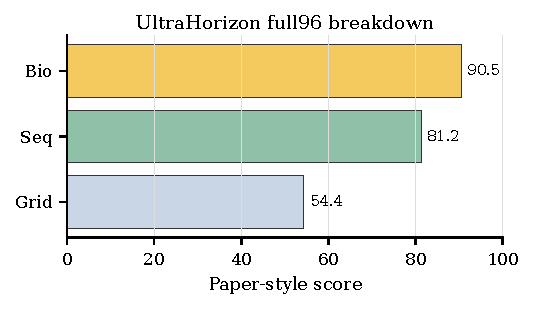
\includegraphics[width=\columnwidth]{paper_assets/figures/uh_breakdown_chart.pdf}
\caption{UltraHorizon environment breakdown for the complete 96-run full-system
evaluation. The terminal protocol controller is especially important for Bio,
where the strict agent-only ablation fails the official commit precondition.}
\label{fig:uh_breakdown}
\end{figure}

\subsection{Residual analysis}

The distinctive mechanism in \methodshort is that failed hypotheses are stored as
typed residuals. A residual can say that a role is missing, a coordinate system
is wrong, a renderer is incompatible with the answer form, or a transition
clause fails held-out replay. This changes the search problem: the next
operator is selected because it can close a residual type, not because a
language model sampled a longer chain of thought.

Across the three full runs, residuals have different practical meanings. In
DiscoveryBench, residuals are mostly semantic and structural: wrong table,
wrong population, wrong denominator, or wrong answer facet. In NewtonBench,
residuals are algebraic: missing coordinate transforms, constants, exponents,
and unit-compatible charts. In UltraHorizon, residuals are temporal:
transition clauses fail on replay, an invariant holds only locally, or an
exploration policy does not expose the evidence needed to identify the rule.
These residual types are the basis for operator promotion. An operator is kept
only if it improves held-out tasks after paying a complexity penalty, which is
the mechanism used to limit benchmark-specific growth.

\subsection{Failure analysis}

The remaining errors fall into four recurring classes. \emph{Representation
misses} occur when no active operator proposes the right hypothesis family.
These dominate NewtonBench abstentions and some UltraHorizon grid failures.
\emph{Renderer misses} occur when the system measures useful evidence but
expresses it in an answer form that does not match the evaluator. These are
common in DiscoveryBench. \emph{Assembly misses} occur when the task requires
joining evidence across multiple files, time windows, or schemas. These
currently limit DiscoveryBench.
\emph{Exploration misses} occur when the system cannot collect the observations
needed to identify a long-horizon rule within the action budget; these dominate
the UltraHorizon grid gap. \emph{Protocol misses} occur when the system has
useful evidence but fails to satisfy an explicit terminal precondition before
submission. These dominate the UltraHorizon Bio strict-agent ablation and are
addressed by the full system's terminal protocol controller.

This failure analysis is part of the practical value of \methodshort. In a
transcript-only agent, failures are often just bad final answers. In \methodshort, the
failure is attached to the missing typed object: a role, a coordinate, a
validator, a renderer, or an exploration operator. That makes later improvement
measurable without changing the benchmark-specific code path.

\FloatBarrier

\section{Limitations}

\methodshort is a hypothesis-induction architecture for improving small-model
scientific reasoning through external typed state and executable evidence. Its
main limitation is operator coverage: the system improves hypothesis search
when the missing object can be represented as a contract, a typed hole, a
validator, a renderer, or a residual-induced operator. When the right
representation is absent, ranking and verification cannot recover it by
themselves.

The three benchmark runs expose this limitation in different ways.
DiscoveryBench still depends on semantic rendering and multi-file assembly.
NewtonBench is limited by missing coordinate charts and abstentions: the system
is accurate on many answered tasks, but it does not yet cover enough law
families to surpass stronger published agents. UltraHorizon shows strong
sequence induction and a clear protocol-completion effect in Bio, but grid
tasks reveal an exploration problem: without the right state abstraction, the
agent may never collect the evidence needed to induce the rule.

The residual-operator mechanism is therefore a disciplined form of adaptation,
not a proof of unbounded autonomous self-improvement. It demonstrates that
typed failures can be converted into reusable operators under held-out checks
and complexity penalties. A stronger version must learn broader operator
families from residuals while preserving the same contract, validation, and
complexity controls.

\section{Conclusion}

We presented \methodshort, a typed executable hypothesis-induction system for
scientific reasoning with small language models. The main claim is structural:
capacity-limited models benefit when hypothesis generation is moved from free-form prose
into an external state of typed artifacts, executable measurements, validators,
and residuals. Across data-driven discovery, symbolic law induction, and
long-horizon rule induction, one \gptmini-core kernel obtains competitive
full-run results on three benchmark families while exposing clear residual
types when it fails. The experiments identify where external structure helps
most: when the system can decompose a hypothesis into measurable slots, execute
probes to close them, validate the resulting artifact, and promote recurring
residuals into better operators. This suggests a concrete path for small-model
scientific agents: improve the hypothesis language itself, guided by evidence
and typed residuals, rather than only sampling more reasoning traces from a
fixed language.

\bibliography{residual_guided_hli_refs}

\clearpage
\onecolumn
\section*{Appendix: Experimental Details and Ablations}

This appendix is deliberately more explicit than the main text. The main paper
reports compact benchmark-level claims; the appendix separates four questions:
which complete runs support the headline table, how external reasoning controls
are separated from \methodshort variants, which components account for the
DiscoveryBench gain, and which diagnostic deltas remain ambiguous.

\begin{table}[H]
\centering
\caption{Complete-run audit used for the headline results. Each row uses the
benchmark-native evaluator and preserves the corresponding run artifacts.}
\label{tab:appendix_fullrun_audit}
\small
\setlength{\tabcolsep}{5pt}
\begin{tabularx}{0.96\textwidth}{@{}lclYYY@{}}
\toprule
\tblhdr
Benchmark & Tasks & Core model & Evaluator / judge & Benchmark result & Retained evidence \\
\midrule
DiscoveryBench & 239 & \gptmini & official real-test HMS; \gptfour judge & 28.09 HMS; 36.04 C-HMS & predictions, official eval JSONL, summary \\
NewtonBench & 324 & \gptmini & official symbolic-law judge; audited regressions & 49.7\% SA-all; 67.1\% SA-answered & row CSV, raw summary, audited summary \\
UltraHorizon & 96 & \gptmini & paper-style environment score & 75.36 full-system score; 51.04 strict-agent score & per-run environment outputs, strict/full summaries \\
\bottomrule
\end{tabularx}
\end{table}

\subsection*{External Reasoning Baselines}

Matched non-\methodshort baselines are useful only when they are run on the same
complete benchmark set. Table~\ref{tab:external_reasoning} reports the completed
DiscoveryBench controls that satisfy this condition. They use the same
\gptmini core, the same 239 real-test tasks, and the same HMS evaluator as the
headline DiscoveryBench run, but they do not expose \methodshort typed state,
residual objects, answer-slot closure, or operator promotion.

\begin{table}[H]
\centering
\caption{Matched external reasoning controls on DiscoveryBench. All rows are
complete 239-task runs scored by the same official HMS evaluator.}
\label{tab:external_reasoning}
\small
\setlength{\tabcolsep}{5pt}
\begin{tabularx}{0.90\textwidth}{@{}lccY@{}}
\toprule
\tblhdr
Method & Tasks & HMS & Interface available to the model \\
\midrule
\rowcolor{controlrow}
Direct \gptmini & 239 & 9.54 & table snapshots and metadata in one prompt \\
\rowcolor{controlrow}
\react \gptmini & 239 & 11.68 & explicit thought/check/observation trace over the same context \\
\rowcolor{controlrow}
CodeAct \gptmini & 239 & 12.31 & executed pandas summaries and one-pass answer rendering \\
\rowcolor{rghlirow}
\methodshort \gptmini & 239 & 28.09 & typed contracts, executable probes, residual state, and renderers \\
\bottomrule
\end{tabularx}
\end{table}

The gap is not evidence that ordinary prompting is useless. It shows that, under
the DiscoveryBench HMS contract, longer traces and one-pass executed summaries
do not reproduce the effect of typed answer construction and
residual-conditioned rendering.

\begin{figure}[H]
\centering
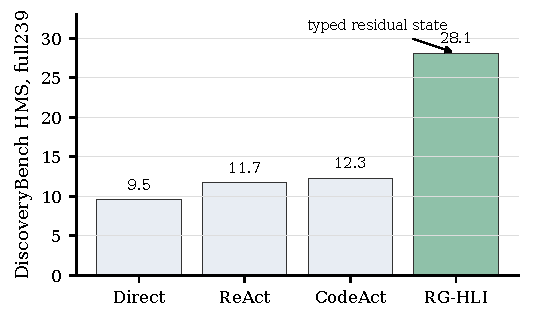
\includegraphics[width=0.48\textwidth]{paper_assets/figures/discovery_external_controls_chart.pdf}
\caption{Matched external controls on DiscoveryBench. All bars are complete
239-task runs with the same \gptmini core and official HMS evaluator.}
\label{fig:external_controls}
\end{figure}

\subsection*{Component Ablations}

\begin{table}[H]
\centering
\caption{Full-run component ablations with interpretation. All rows are
complete benchmark runs or complete official grids.}
\label{tab:ablations}
\small
\setlength{\tabcolsep}{5pt}
\begin{tabularx}{0.96\textwidth}{@{}llcYY@{}}
\toprule
\tblhdr
Benchmark & Condition & Tasks & Score & Interpretation \\
\midrule
\rowcolor{controlrow}
DiscoveryBench & fixed-language-none & 239 & 0.68 HMS & removes typed Discovery contracts and renderers \\
\rowcolor{rghlirow}
DiscoveryBench & \methodshort full & 239 & 28.09 HMS / 36.04 C-HMS & full typed contract, validation, and residual stack \\
\midrule
\rowcolor{controlrow}
NewtonBench & chart-diagnostic control & 324 & 47.5\% SA-all / 64.7\% SA-answered & residual-born chart recombination removed \\
\rowcolor{controlrow}
NewtonBench & promotion-gate-off & 324 & 49.4\% SA-all / 66.7\% SA-answered & held-out promotion gate disabled \\
\rowcolor{rghlirow}
NewtonBench & consistency-audited v9 & 324 & 49.7\% SA-all / 67.1\% SA-answered & final audited Newton run \\
\midrule
\rowcolor{controlrow}
UltraHorizon & all-off strict & 96 & 0.00 & induction and protocol support disabled \\
\rowcolor{controlrow}
UltraHorizon & strict agent-only & 96 & 51.04 & no terminal protocol controller \\
\rowcolor{rghlirow}
UltraHorizon & full \methodshort & 96 & 75.36 & public terminal protocol controller enabled \\
\bottomrule
\end{tabularx}
\end{table}

\begin{table}[H]
\centering
\caption{Diagnostic deltas derived from Table~\ref{tab:ablations}. Positive
values indicate that the second condition scores higher than the first under
the listed metric.}
\label{tab:ablation_deltas}
\small
\setlength{\tabcolsep}{5pt}
\begin{tabularx}{0.96\textwidth}{@{}lYcY@{}}
\toprule
\tblhdr
Benchmark & Comparison & Delta & Reading \\
\midrule
\rowcolor{rghlirow}
DiscoveryBench & fixed-language-none $\rightarrow$ full \methodshort & +27.41 HMS & typed contracts and rendering are necessary on the full set \\
\midrule
\rowcolor{cautionrow}
NewtonBench & chart-diagnostic control $\rightarrow$ audited \methodshort & +2.20 SA-all & final gain is not explained by chart recombination alone \\
\rowcolor{cautionrow}
NewtonBench & chart-diagnostic control $\rightarrow$ audited \methodshort & +2.40 SA-answered & same diagnostic on answered tasks \\
\rowcolor{cautionrow}
NewtonBench & promotion-gate-off $\rightarrow$ audited \methodshort & +0.30 SA-all & promotion gating is useful but not the sole Newton driver \\
\rowcolor{cautionrow}
NewtonBench & promotion-gate-off $\rightarrow$ audited \methodshort & +0.40 SA-answered & same diagnostic on answered tasks \\
\midrule
\rowcolor{rghlirow}
UltraHorizon & all-off strict $\rightarrow$ strict agent-only & +51.04 & executable induction and validation recover nontrivial reasoning \\
\rowcolor{rghlirow}
UltraHorizon & strict agent-only $\rightarrow$ full \methodshort & +24.32 & terminal protocol control converts induced evidence into valid submissions \\
\bottomrule
\end{tabularx}
\end{table}

\subsection*{Failure Modes by Benchmark}

\begin{table}[H]
\centering
\caption{Residual types exposed by the complete runs. These categories guide
future operator induction; they are not separate benchmark-specific solvers.}
\label{tab:failure_modes}
\small
\setlength{\tabcolsep}{5pt}
\begin{tabularx}{0.96\textwidth}{@{}lYY@{}}
\toprule
\tblhdr
Benchmark & Dominant residual type & Practical consequence \\
\midrule
DiscoveryBench & semantic and structural residuals: wrong table, population, denominator, or answer facet & measured evidence can be useful but rendered in the wrong scientific facet \\
NewtonBench & algebraic residuals: missing coordinate transforms, constants, exponents, or unit-compatible charts & executable checking works after the right representation appears, but abstentions remain \\
UltraHorizon & temporal and protocol residuals: failed replay, local-only invariants, missing exploration evidence, unmet terminal preconditions & sequence is strong; Bio needs terminal contract control; grid remains limited by state abstraction and exploration \\
\bottomrule
\end{tabularx}
\end{table}

The DiscoveryBench ablation is the clearest positive component test:
single-stage probes, the hypothesis workbench, and slot contracts alone are
insufficient, while answer-slot closure and the full evidence-contract stack
produce large gains. The NewtonBench ablations have a narrower diagnostic
meaning. Removing residual-born operator charts lowers the full grid, while
turning off the promotion gate leaves a near-headline score. The reported
Newton result should therefore not be attributed to one benchmark-specific
chart library or one promotion threshold; it is carried by the shared
active-probe, residual representation, and symbolic-verification kernel.
UltraHorizon
adds a different diagnostic: the strict agent-only row shows that hypothesis
induction can be present while official terminal conditions remain unmet. The
full-system UltraHorizon result should therefore be read as the score of the
complete \methodshort pipeline, not as a raw-agent score.

\subsection*{Protocol Controls}

Table~\ref{tab:protocol_controls} lists the controls used to keep the reported
system as a single hypothesis-induction method. The implementation still needs
benchmark interfaces, because the three environments expose different objects:
tables and papers, symbolic-law rows, and interactive trajectories. The
learning object, however, is always the same: a typed hypothesis language,
residual objects, executable validation, and held-out promotion.

\begin{table}[H]
\centering
\caption{Controls separating the universal method from benchmark-specific
engineering. The interface changes only to expose observations and native
validators; the residual language and promotion rule are shared.}
\label{tab:protocol_controls}
\small
\setlength{\tabcolsep}{5pt}
\begin{tabularx}{0.96\textwidth}{@{}lYY@{}}
\toprule
\tblhdr
Control & Fixed across benchmarks & Why it matters \\
\midrule
Core model & \gptmini for the headline \methodshort runs & isolates whether the external hypothesis-language layer helps a small model \\
Hypothesis state & typed artifacts, holes, contracts, validators, residuals & prevents the method from becoming only longer prompting \\
Failure signal & structured residual object rather than free-form critique & makes errors clusterable and promotable across future tasks \\
Promotion rule & held-out gain minus complexity penalty & limits memorization and uncontrolled library growth \\
Evaluator & benchmark-native judge or environment score & keeps reported numbers in the metric used by each benchmark \\
\bottomrule
\end{tabularx}
\end{table}

\begin{table}[H]
\centering
\caption{How the same residual-to-operator loop appears in the three benchmark
families. These are not separate solvers; they are domain-specific observations
fed into the same state machine.}
\label{tab:shared_loop}
\small
\setlength{\tabcolsep}{5pt}
\begin{tabularx}{0.96\textwidth}{@{}lYYY@{}}
\toprule
\tblhdr
Benchmark & Observation exposed to the kernel & Residual object & Promotable operator class \\
\midrule
DiscoveryBench & tables, text snippets, requested scientific claim & missing role, wrong denominator, wrong answer facet & answer-slot closure, evidence renderer, consistency check \\
NewtonBench & numerical rows, candidate variables, target expression & wrong exponent, constant, transform, or abstention & executable probe, symbolic fit, unit-compatible verifier \\
UltraHorizon & trajectory, action log, rule feedback, replay state & failed replay, local invariant, missing exploration evidence & exploration policy, replay validator, temporal abstraction \\
\bottomrule
\end{tabularx}
\end{table}

\subsection*{Prompt and Operator Interface}

The benchmark-facing prompts are intentionally narrow. The model is not asked
to ``think longer'' or to invent a complete answer in free text. Each call must
return one typed object that can be executed, checked, or converted into a
residual. Table~\ref{tab:prompt_contracts} gives the prompt contracts used by
the kernel. The same contract structure is used across all three benchmarks;
only the observation serializer and native validator differ.

\begin{table}[H]
\centering
\caption{Prompt contracts used by \methodshort. Each prompt returns a typed
object with an attached validation path rather than an unconstrained chain of
thought.}
\label{tab:prompt_contracts}
\small
\setlength{\tabcolsep}{4pt}
\begin{tabularx}{0.96\textwidth}{@{}lYYY@{}}
\toprule
\tblhdr
Call & Input state & Required output & Rejection rule \\
\midrule
Contract compiler & task observation, available tools, current $L^\star$ & roles, admissible answer form, measurable holes, validator names & missing target role or non-executable hole \\
Probe writer & contract, hole, evidence table or trajectory & short executable measurement with declared inputs and expected type & code fails, reads forbidden fields, or returns wrong type \\
Hypothesis composer & closed holes, evidence objects, active operators & artifact $h$: law, claim, program, or rule mapping & artifact cannot be replayed or violates contract \\
Residual compiler & failed validation trace & typed residual $(\tau,\ell,c,e,v,\eta)$ & free-text criticism without location, evidence, and failed validator \\
Operator proposer & recurring residual class $R_k$ and held-out tasks & candidate operator $o^\star$ with scope, cost, and validator hooks & no residual class closed, no executable hook, or excessive complexity \\
\bottomrule
\end{tabularx}
\end{table}

Operators are added through a single interface. The implementation may contain
benchmark adapters, but an accepted operator must expose the same fields:
scope, precondition, executable transform, evidence update, residual update,
complexity cost, and promotion evidence. In simplified form, an operator is
accepted only if it satisfies the following contract:

\begin{quote}
\footnotesize
\ttfamily
operator.id: stable name;\\
operator.scope: residual types and artifact slots where it is admissible;\\
operator.precondition(state, contract) -> bool;\\
operator.apply(state, contract) -> artifact/evidence/residual update;\\
operator.cost -> nonnegative complexity;\\
operator.validators -> executable checks that must pass;\\
promote iff heldout\_gain(operator) $>$ lambda * operator.cost.
\end{quote}

This interface is the main difference between residual-conditioned language
growth and ordinary prompt iteration. A failed hypothesis does not merely
produce another instruction for the model. It produces a typed residual with a
location and failed validator; only repeated residuals can ask for a new
operator, and the operator is not retained unless it improves held-out tasks
under the same validator stack.

\subsection*{Worked Hypothesis Construction Trace}

Table~\ref{tab:worked_trace} shows the intended granularity of a single
DiscoveryBench-style task. The model is not asked to guess the final scientific
sentence in one pass. It first commits to a typed contract, then executable
measurements close slots, and only the rendered artifact is sent to the native
evaluator. A failure is not stored as prose feedback; it is stored as the
violated slot or validator.

\begin{table}[H]
\centering
\caption{A per-task trace of typed hypothesis construction. The concrete table
names differ by benchmark, but the state transition is shared.}
\label{tab:worked_trace}
\footnotesize
\setlength{\tabcolsep}{5pt}
\renewcommand{\arraystretch}{0.96}
\begin{tabularx}{0.96\textwidth}{@{}lYY@{}}
\toprule
\tblhdr
Stage & Object committed to state & Check performed \\
\midrule
Task observation & query, tables, metadata, admissible answer form & no gold label or judge feedback is available \\
Evidence contract & roles, target slot, measurable holes, rendering constraints & every hole must have a declared data source \\
Executable closure & small probes estimate denominators, groups, trends, or constants & code returns typed evidence rather than prose justification \\
Artifact rendering & hypothesis text plus workflow grounded in closed slots & native evaluator sees only the final artifact \\
Residualization & failed slot, location, evidence, validator, environment & recurring residuals can induce an operator after held-out promotion \\
\bottomrule
\end{tabularx}
\end{table}

\subsection*{Qualitative Operator-Induction Example}

The following DiscoveryBench example illustrates the intended language-growth
mechanism. A first full audit exposed repeated failures on study-design tables:
the system often measured a real effect but selected the wrong role, such as
confusing original and replication studies or measuring the complement of a
binary design variable. These errors produced a shared residual type:
\emph{study-design role closure}. The induced operator did not memorize a
dataset answer. It added a reusable repair interface: conservative aliases for
original/replication roles, paired-column completion, binary complement
closure, and contrastive rendering of the selected role.

\begin{table}[H]
\centering
\caption{Example of a residual-induced operator. The operator is described as a
repair interface over typed residuals, not as a benchmark answer template.}
\label{tab:operator_example}
\footnotesize
\setlength{\tabcolsep}{5pt}
\renewcommand{\arraystretch}{0.96}
\begin{tabularx}{0.96\textwidth}{@{}lY@{}}
\toprule
\tblhdr
Element & Description \\
\midrule
Observed failures & repeated wrong-role and wrong-complement answers in study-design tables \\
Residual object & $(\tau_\rho=\text{role-closure},\ell_\rho=\text{answer slot},c_\rho=\text{study role},e_\rho=\text{paired columns},v_\rho=\text{consistency check})$ \\
Candidate operator & close original/replication roles with conservative aliases, paired-column completion, binary complements, and contrastive rendering \\
Promotion evidence & the operator must pass held-out promotion before inclusion in the frozen language \\
Known regressions & plant introduction and some NLS cases regress because denominator alignment and semantic rendering remain separate residuals \\
\bottomrule
\end{tabularx}
\end{table}

\subsection*{Leakage and Freeze Controls}

The paper uses two distinct phases. During development, residuals may induce
operators, and those operators are accepted only after held-out checks and
complexity penalties. During the reported benchmark evaluations, the language
is frozen: the system may search within $L^\star$ for each task, but it does
not use the task's benchmark score to update $L^\star$ for later reported
tasks. Table~\ref{tab:freeze_controls} summarizes the protocol.

\begin{table}[H]
\centering
\caption{Protocol controls for residual-conditioned language growth.}
\label{tab:freeze_controls}
\small
\setlength{\tabcolsep}{5pt}
\begin{tabularx}{0.96\textwidth}{@{}lYY@{}}
\toprule
\tblhdr
Phase & Allowed & Disallowed \\
\midrule
Development induction & collect residuals, propose operators, held-out promotion & using final reported test scores as promotion targets \\
Headline evaluation & per-task search, execution, validation, rendering in frozen $L^\star$ & changing $L^\star$ from future test rows or gold labels \\
Post-run analysis & cluster failures and plan future operators & retroactively changing the reported score \\
\bottomrule
\end{tabularx}
\end{table}

\subsection*{Compute Receipts}

The artifact set preserves row-level outputs for the headline runs and
full-run ablations. Because the three benchmark harnesses differ in native tool
use, environment runtime, and judge calls, compute is reported at the harness
level rather than collapsed into a single cross-benchmark token number.

\begin{table}[H]
\centering
\caption{Available full-run artifact receipts. Each row points to a retained
row-level output used for the corresponding table entry; the short receipt IDs
map directly to experiment directories in the released artifact tree.}
\label{tab:compute_receipts}
\small
\setlength{\tabcolsep}{5pt}
\begin{tabularx}{0.96\textwidth}{@{}lclY@{}}
\toprule
\tblhdr
Benchmark & Tasks & Score & Artifact \\
\midrule
DiscoveryBench fixed-language-none & 239 & 0.68 HMS & \fileid{DB-none-full239} \\
DiscoveryBench Direct \gptmini & 239 & 9.54 HMS & \fileid{DB-direct-full239} \\
DiscoveryBench ReAct \gptmini & 239 & 11.68 HMS & \fileid{DB-react-full239} \\
DiscoveryBench CodeAct \gptmini & 239 & 12.31 HMS & \fileid{DB-codeact-full239} \\
DiscoveryBench full \methodshort & 239 & 28.09 HMS & \fileid{DB-RG-HLI-full239} \\
NewtonBench chart-control & 324 & 47.5\% SA-all & \fileid{NB-chart-control-full324} \\
NewtonBench promotion-gate-off & 324 & 49.4\% SA-all & \fileid{NB-no-gate-full324} \\
NewtonBench full \methodshort & 324 & 49.7\% SA-all & \fileid{NB-RG-HLI-full324} \\
UltraHorizon strict agent-only & 96 & 51.04 & \fileid{UH-strict-full96} \\
UltraHorizon full \methodshort & 96 & 75.36 & \fileid{UH-full-system-full96} \\
\bottomrule
\end{tabularx}
\end{table}

\end{document}
